% ------------------------------------------------- %
% ---   NAGŁÓWEK - PROSZĘ NIE ZMIENIAĆ USTAWIEŃ --- %
% ------------------------------------------------- %
\documentclass[a4paper,10pt]{article}
\usepackage[utf8]{inputenc}
\usepackage[T1]{fontenc}
% Zamiast: \usepackage[margin=1.8cm]{geometry}
\usepackage[margin=1cm, top=1.4cm, headsep=0.3cm]{geometry}
\usepackage{tabularx}
\usepackage{booktabs}
\usepackage{fontawesome5}
\usepackage{amsmath,amssymb}
\usepackage[table]{xcolor}
\usepackage{graphicx}
\usepackage{fancyhdr}

\definecolor{tableheader}{RGB}{230, 238, 248}
\definecolor{scorebg}{RGB}{205, 222, 242}
\definecolor{primaryblue}{RGB}{30, 75, 140}

\pagestyle{fancy}
\fancyhf{}
\lhead{\small \textbf{Projekt 1} -- Wstęp do Uczenia Maszynowego 2026Z}
\rhead{\small Raport KM1}
\renewcommand{\headrulewidth}{0.4pt}

% ------------------------------------------------------ %
% --- KONIEC NAGŁÓWKA - PROSZĘ NIE ZMIENIAĆ USTAWIEŃ --- %
% ------------------------------------------------------ %

\begin{document}


\vspace{-1em}
\noindent
\renewcommand{\arraystretch}{1.3}
\begin{tabularx}{\textwidth}{|>{\hsize=1.2\hsize}X|>{\hsize=0.8\hsize}X|>{\centering\arraybackslash}m{2.5cm}|}
\hline
\rowcolor{tableheader}

% ----------------------------------------------------------- %
% ---   PROSZĘ UZUPEŁNIĆ TABELĘ W LINIJKACH Z KOMENTARZEM --- %
% ----------------------------------------------------------- %

\textbf{Imię i Nazwisko:} Błażej Klepacki
& \textbf{Kierunek:} MAD % ZOSTAW WŁAŚCIWE
& \cellcolor{scorebg}\textbf{PUNKTACJA} \\
\rowcolor{tableheader}
\textbf{Prowadzący:}  AK % ZOSTAW WŁAŚCIWE
& \textbf{Numer albumu:} 331389 
& \cellcolor{scorebg}\huge{\textbf{ / 8}} \\
\hline
\end{tabularx}
\renewcommand{\arraystretch}{1.0}

\vspace{-1em}


\section*{\color{primaryblue}Raport z Kamienia Milowego 1: Eksploracja i przygotowanie danych}

% ----------------------- %
% ---  TREŚĆ RAPORTU  --- %
% ----------------------- %

\section{Eksploracyjna analiza danych}

Zbiór treningowy ma 6400 obserwacji i 23 cechy (bez duplikatów), a testowy 1600 obserwacji. Zmienna docelowa to zwłoka w płatności w kolejnym miesiącu, która dotyczy 21,6\% klientów (1381 z 6400), więc klasy są niezbalansowane. \texttt{SEX}, \texttt{EDUCATION} i \texttt{MARRIAGE} są kategoryczne (zapisane jako liczby), a pozostałe cechy liczbowe. Kwoty (\texttt{BILL\_AMT}, \texttt{PAY\_AMT}) mają mocno prawoskośne rozkłady, a w \texttt{PAY\_*} większość wartości to $-2$, $-1$ lub $0$ (w \texttt{PAY\_0} około 78\%). Wartości dodatnie \texttt{PAY\_*} oznaczają opóźnienie w miesiącach (tak jest w oryginalnym zbiorze UCI, w poleceniu nie jest to rozpisane).

\subsection{Braki danych}

Braki są w trzech kolumnach: \texttt{PAY\_5} (9,9\%), \texttt{BILL\_AMT6} (10,2\%) i \texttt{PAY\_AMT4} (9,9\%). Razem dotyczą 27\% wierszy (1743 z 6400), więc usuwanie wierszy z brakami odpada. Braki nie są ze sobą skorelowane (korelacja wskaźników braków około 0), a odsetek zwłok jest podobny z brakiem i bez niego (0,22--0,24 wobec 0,21--0,22), więc nie widać zależności od zmiennej docelowej i wyglądają na losowe. W zbiorze testowym braki są w tych samych kolumnach i w podobnej skali (9--10\%). Uzupełnieniem zajmę się w pipeline w KM2.

\subsection{Wartości odstające}

Według reguły $1{,}5\cdot IQR$ poza wąsami boxplota jest 8--9\% obserwacji w każdej kolumnie \texttt{BILL\_AMT} i \texttt{PAY\_AMT} (w \texttt{LIMIT\_BAL} 1\%, w \texttt{AGE} 0,5\%). Skrajne kwoty wyglądają na prawdziwe, duże wartości, więc ich nie usuwam (drzewa są odporne na wartości skrajne). Bardziej podejrzane są wartości ujemne: wpłata nie powinna być ujemna, a \texttt{PAY\_AMT} ma ich 920--1219 w każdej kolumnie (co najmniej jedna w 57\% wierszy). Ujemny jest też jeden \texttt{LIMIT\_BAL} oraz 833--936 wartości w każdej kolumnie \texttt{BILL\_AMT}, co przy rachunkach może być nadpłatą. Możliwe, że to szum w danych, więc decyzję podejmę w KM2. Dodatkowo \texttt{PAY\_3} ma jedną obserwację równą $-3$ (w innych \texttt{PAY\_*} minimum to $-2$), a \texttt{EDUCATION} (0, 4, 5, 6) i \texttt{MARRIAGE} (0, 3) mają rzadkie wartości oznaczające ,,inne'' (108 i 75 obserwacji).

\subsection{Relacje i istotność zmiennych}

Ze zmienną docelową najsilniej skorelowana jest historia spłat: \texttt{PAY\_0} (0,31), \texttt{PAY\_2} (0,26) i kolejne \texttt{PAY\_*} (malejąco do 0,17), a z kwot tylko \texttt{LIMIT\_BAL} ($-0{,}15$). Drzewo o głębokości 5 daje podobny obraz: istotność \texttt{PAY\_0} to 0,625, \texttt{PAY\_2} 0,127, a każdej z pozostałych cech poniżej 0,035. Odsetek zwłok rośnie z opóźnieniem: 11--18\% dla \texttt{PAY\_0} $\le 0$, 32\% dla 1 i około 68\% dla 2 i 3 (rys.~\ref{fig:grupy}). Zmienne demograficzne mają słaby związek ze zmienną docelową (np. 24\% zwłok u mężczyzn i 20\% u kobiet). Kolumny \texttt{BILL\_AMT} mają z $y$ korelację około 0, za to są silnie skorelowane między sobą (0,79--0,94), czyli współliniowe, co może przeszkadzać modelom liniowym w KM2.

\begin{figure}[!htb]
\centering
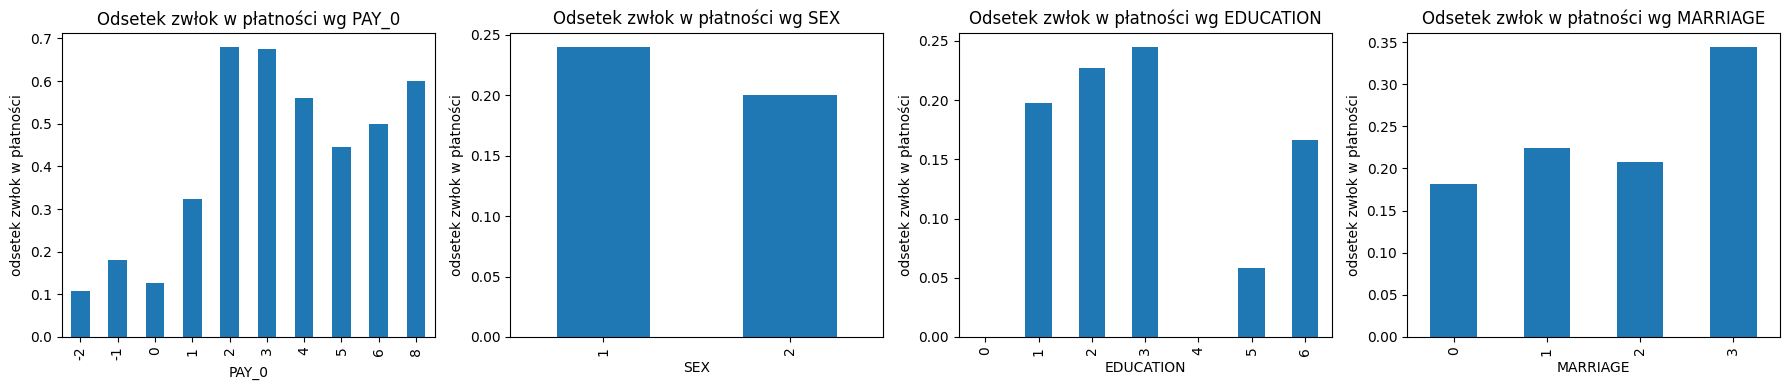
\includegraphics[width=\textwidth]{fig_grupy.png}
\caption{Odsetek zwłok w płatności w grupach wg \texttt{PAY\_0}, \texttt{SEX}, \texttt{EDUCATION} i \texttt{MARRIAGE}.}
\label{fig:grupy}
\end{figure}



\section{Metryka ewaluacji i podział danych}

Zadanie to klasyfikacja binarna, a wynikiem końcowym ma być wektor prawdopodobieństw klasy 1, więc potrzebuję metryki, która ocenia prawdopodobieństwa, a nie same etykiety. Jako główną metrykę wybieram \textbf{ROC AUC}: krzywa ROC to pary $(FPR, TPR)$ dla kolejnych progów odcięcia, a AUC to pole pod nią (0,5 dla klasyfikatora losowego, 1 dla idealnego). Nie zależy od progu i mówi, jak dobrze model układa klientów od najmniej do najbardziej ryzykownych. Klasy są niezbalansowane (21,6\% klasy 1), więc accuracy jest mylące: klasyfikator, który zawsze zgaduje klasę 0, ma accuracy 0,784, ale AUC 0,5 i F1 równe 0. Pomocniczo liczę \textbf{average precision} (AP), bo jest czulsza, gdy klasa pozytywna jest rzadka, a losowy klasyfikator ma AP równe udziałowi klasy 1 (0,216). Accuracy podaję tylko dla porównania.

\subsection{Strategia podziału danych}

Zbiór \texttt{X\_test} nie ma etykiet, więc nie da się na nim niczego ocenić. Dlatego z \texttt{X\_train} wydzieliłem 20\% obserwacji jako zbiór hold-out (1280 obserwacji), stratyfikowany względem $y$, żeby udział klasy 1 był wszędzie taki sam (21,6\%). Hold-out nie służy do doboru hiperparametrów ani modelu, użyję go tylko do końcowej oceny wybranego modelu. Eksploracyjna analiza była robiona na całym \texttt{X\_train}, ale nie służyła do wyboru modelu ani hiperparametrów. Na pozostałych 80\% (5120 obserwacji) dobieram hiperparametry 5-krotną stratyfikowaną walidacją krzyżową (w każdym foldzie 4096 obserwacji uczących i 1024 walidacyjnych, udział klasy 1 wszędzie 21,6\%). Wybrałem CV zamiast jednego podziału walidacyjnego, bo pojedynczy podział daje niestabilne wyniki (zauważone na lab 2), a stratyfikację dodałem ze względu na niezbalansowanie klas. Wszystkie \texttt{random\_state} wynoszą 123, więc wyniki się powtarzają.


\section{Optymalizacja hiperparametrów modelu drzewa}

Domyślne drzewo się przeucza: ROC AUC wynosi 1,0 na zbiorze uczącym, a w CV tylko 0,61. Wybrałem trzy hiperparametry ograniczające jego złożoność: \texttt{max\_depth} (maksymalna głębokość), \texttt{min\_samples\_leaf} (minimalna liczba obserwacji w liściu) i \texttt{ccp\_alpha} (kara za złożoność w przycinaniu cost-complexity). Najpierw sprawdziłem każdy z nich osobno, przy pozostałych domyślnych (rys.~\ref{fig:hiper}): ROC AUC w CV rośnie do maksimum, a potem spada, natomiast na zbiorze uczącym rośnie wraz ze złożonością drzewa, czyli rośnie przeuczenie. Na tej podstawie ustaliłem siatkę: \texttt{max\_depth} $\in \{3,4,5,6,8,10,\text{None}\}$, \texttt{min\_samples\_leaf} $\in \{1,10,30,50,75,100,150,200\}$ i \texttt{ccp\_alpha} $\in \{0,\,10^{-4},\,3\cdot10^{-4},\,5\cdot10^{-4},\,10^{-3},\,2\cdot10^{-3}\}$. Daje to 336 kombinacji, a każdą oceniłem 5-krotną stratyfikowaną CV (ROC AUC, pomocniczo AP). Wartości są gęściej tam, gdzie krzywe osobne mają maksimum.

\begin{figure}[!htb]
\centering
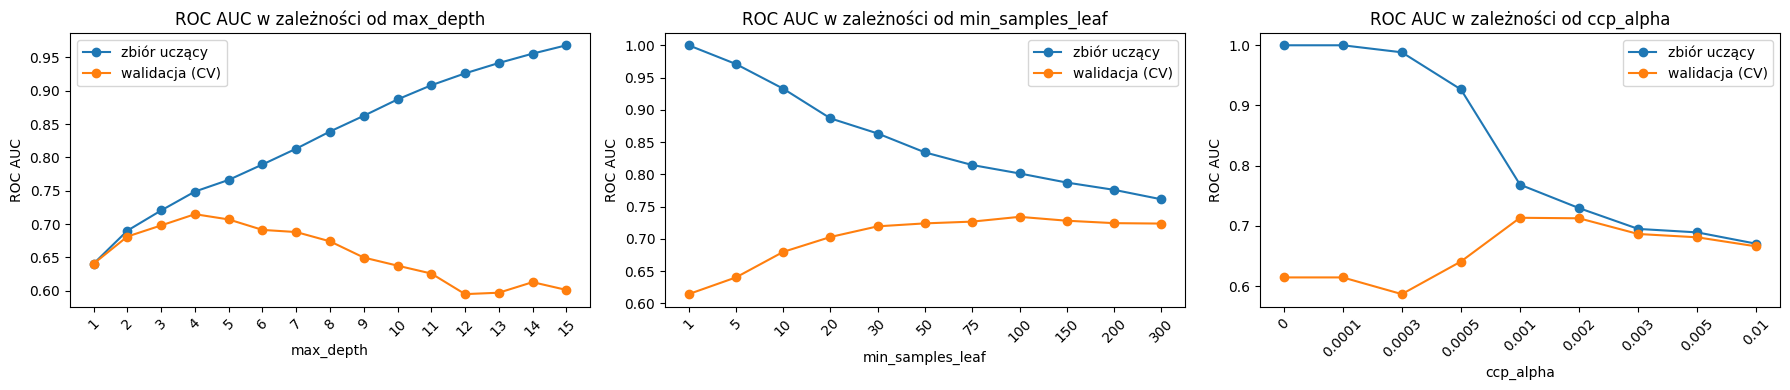
\includegraphics[width=\textwidth]{fig_hiperparametry.png}
\caption{ROC AUC na zbiorze uczącym i w CV w zależności od każdego hiperparametru osobno.}
\label{fig:hiper}
\end{figure}

Najlepsza kombinacja to \texttt{max\_depth=8}, \texttt{min\_samples\_leaf=75}, \texttt{ccp\_alpha=0,0003} (CV ROC AUC 0,736 $\pm$ 0,013, AP 0,490). Najlepsze kombinacje różnią się o mniej niż 0,003, czyli mniej niż odchylenie standardowe między foldami (0,01--0,02), więc wybór wśród nich jest w dużej mierze przypadkowy. Osobno najwięcej poprawia \texttt{min\_samples\_leaf} (z około 0,61 do około 0,73), ale w siatce różne kombinacje dają podobny wynik, bo każdy hiperparametr ogranicza złożoność na swój sposób. Zbyt duże \texttt{ccp\_alpha} (od 0,001) i zbyt płytkie drzewo (\texttt{max\_depth}=3, najlepiej 0,706) obniżają wynik. Na hold-oucie wybrane drzewo (głębokość 8, 26 liści) daje ten sam ROC AUC co w CV, więc nie widać przeuczenia przy doborze hiperparametrów:

\begin{center}
\small
\begin{tabular}{lccccc}
\toprule
Model & CV ROC AUC & CV AP & hold-out ROC AUC & hold-out AP & hold-out accuracy \\
\midrule
domyślne drzewo & 0,614 & 0,286 & 0,602 & 0,275 & 0,724 \\
drzewo po tuningu & 0,736 & 0,490 & 0,736 & 0,469 & 0,812 \\
\bottomrule
\end{tabular}
\end{center}


\section{Podsumowanie i wnioski}

Zbiór ma 6400 obserwacji i niezbalansowane klasy (21,6\% zwłok), a najważniejszym predyktorem jest historia spłat, przede wszystkim \texttt{PAY\_0}. W danych są braki w trzech kolumnach (około 10\%, wyglądają na losowe), ujemne wpłaty (57\% wierszy), rzadkie kategorie ,,inne'' i współliniowe \texttt{BILL\_AMT}, co zostawiam do rozwiązania w pipeline'ie w KM2. Jako metrykę wybrałem ROC AUC (pomocniczo AP), a dane podzieliłem na stratyfikowany hold-out 20\% i 5-krotną stratyfikowaną CV na reszcie. Po strojeniu trzech hiperparametrów drzewo z \texttt{max\_depth=8}, \texttt{min\_samples\_leaf=75} i \texttt{ccp\_alpha=0,0003} ma ROC AUC 0,736 (w CV i na hold-oucie), czyli o około 0,13 więcej niż drzewo domyślne na hold-oucie. Ograniczenia: najlepsze kombinacje różnią się o mniej niż 0,003, więc ich kolejność jest mało pewna, a hold-out ma tylko 1280 obserwacji (około 276 z klasą 1). W KM2 uzupełnię braki, zdecyduję, co zrobić z ujemnymi wpłatami i kategoriami ,,inne'', i dodam drugi model (np. regresję logistyczną z lab 4).

% ------------------------------- %
% ---  KONIEC TREŚCI RAPORTU  --- %
% ------------------------------- %

\end{document}
